\section{Legal Aspects}
\paragraph{}
Whether performing reverse engineering on a digital object is legal or not cannot always be easily answered as regulations differ on a country basis and do not even always have a straight forward answer. Laws such as the fair use in the United States are subject to interpretation and so, can only be answered by the court on a case by case basis. The introductory case of Sega vs Accolade is a perfect example of such situation, where the intermediate copies have been ruled as fair use, but only after appealing the initial judgement.

\paragraph{}
Extraction of knowledge from an artefact can be costly or cheap and time-consuming or fast~\cite{samuelson2002law}. The artefact and these notions are what determine if additional legal protections are necessary. The goal here is not to give an exhaustive list of all of these legal protections because it is not the purpose of this work, but rather to mention some of the main legal doctrines that could prevent a reverser to do his or her job in compliance with the law. The emphasis will be put onto the United States as information on the matter is significantly harder to find for a country such as Belgium. Nevertheless, it can give a general idea of what could get in the way of a reverser.

\subsection{Digital Millennium Copyright Act}
\begin{quotation}
	\noindent ``\emph{To pass laws that regulate the research of technological measures that protect copyrights and the dissemination of such results is to concede that copyright technology is broken and can never be improved — that the only possible outcome of allowing common people to understand copyright control technology is the demise of the technology.}''
	\begin{flushright}\textbf{Andrew Huang, 2003}\end{flushright}
\end{quotation}

\paragraph{} 
For years, copyright industries would sell their products in the form of tangible goods such as books and CDs. The rise of digital technologies opened up a new market for these industries with the possibility to the mass-marketing of contents that are technologically protected. At the same time, these companies pushed the American Congress to implement legal obstacles to protect the technological protections so that it would be illegal to break them. The Digital Millennium Copyright Act, or DMCA for short, is the law which embodies that legal protection~\cite{samuelson2002law}.  

\paragraph{}
According to the Electronic Frontier Foundation, this law does not only prevent breaking protections, but also breaking access controls. They give as example breaking authentication handshakes, code signing, code obfuscation, and protocol encryption~\cite{relawdaq}. The law has nevertheless an exception which allows the development and the use of tools to bypass these protections as long as it stays in the scope of interoperability~\cite{samuelson2002law}.

\subsection{Copyright Law and Fair Use} \label{copyright_law_and_fair_use}
\paragraph{}
Copyright laws give a certain set of exclusive rights for an original work to its creator, the copyright owner. It is some sort of intellectual property that is applied to, but not only, software application. To make copies of a protected product, it is necessary to either have an agreement with the owner or to go through an exception granted by the copyright laws. Copyright does not prevent someone else from reinventing the protected object.

\paragraph{}
Most of the software applications are distributed in the form of digital objects because users don't necessarily care about their source code representations and also because companies behind software want to keep their source code and associated documentation as trade secrets~\cite{litman1992copyright}. Decompilation and disassembly, two major techniques to perform reverse engineering that will be discussed later, could arguably infringe copyright laws as they make intermediate approximate copies of the original source code. 

\paragraph{}
Fair use is one of the exceptions that can be used to make copying a software lawful. It allows a rightful owner of a copy of the software application to copy the work for a purpose and to an extend that will not hurt the owner of the copyright. The following list of factors are used to determine whether a certain application can fall into fair use~\cite{litman1992copyright}:
\begin{itemize}
	\item the defendant's purpose in using the protected work
	\item the nature of the copyrighted work
	\item the amount and substantiality of what is taken
	\item the potential for harm to the market for the protected work
\end{itemize}

\paragraph{}
Two more privileges are given to the owners of copies of copyrighted software. An essential step in launching a software is to copy the digital object into the random access memory (RAM) and then the caches. It is stated that if the copy has been lawfully acquired, that form of reproduction is not unlawful under copyright ground. Backup copies are treated the same way and under the same prerequisite. Copying a software application to reverse engineer it is going beyond these two privileges and might infringed the law if it does not fall into fair use or any other relevant exception~\cite{samuelson1990reverse}.

\subsection{Trade Secret Law}
\paragraph{}
A trade secret is defined by the Uniform Trade Secrets Act as follows:
\begin{framed}
	\begin{definition}
		\underline{Trade secret} means information, including a formula, pattern, compilation, program, device, method, technique, or process, 
		\begin{itemize}
			\item that derives independent economic value, actual or potential, from not being generally known to or readily ascertainable through appropriate means by other persons who might obtain economic value from its disclosure or use; and
			\item is the subject of efforts that are reasonable under the circumstances to maintain its secrecy.
		\end{itemize}
		\begin{flushright}
			\hfill{}{CIVIL CODE SECTION 3426-3426.11~\cite{trade_secret_law}}
		\end{flushright}
	\end{definition}
\end{framed}
\paragraph{}
Trade secret laws only protect from wrongful acquisitions and use or disclosure of trade secrets. An example would be breaching a non disclosure agreement or using industrial espionage. If the intermediate copies are ruled as fair use, obtaining the trade secrets using reverse engineering is in accordance with the law. The gathered information can thereafter be published and or used freely in the eyes of the law~\cite{samuelson1990reverse, samuelson2002law, graham1999legal}.

\paragraph{}
Since trade secrets are not perceived as intellectual properties (i.e a monopoly over something to an owner designated by the law), one might want to consider patenting a discovery. To get a patent, an author has to disclose information containing at least a written description of the discovery and a series of steps to reproduce it. If the patent is accepted, it will fall into the public domain and so render the usage of reverse engineering useless as the knowledge will be freely available for all. In contrast with copyright, patents do prevent artefacts to be reinvented by someone else, but these protections have expiration dates.

\subsection{Contract Law}
\paragraph{}
Software can be sorted into two categories, free and not free software. The \textit{free} has to be interpreted as freedom of speech and not as in free of charge. According to the Free Software Foundation, for a software to be free, it has to give a user the freedom to run, copy, distribute, study, change and improve itself~\cite{stallman2002free}. On the other side, proprietary software strip users from certain liberties that are specified in end-user license agreements, or EULAs for short. When an application comes with a EULA, the reverser has to make sure it does not have a no reverse engineering clause as it legally prevents it. To be noted that the enforceability of these restrictions have been challenged in America as well as in Europe~\cite{samuelson2002law}. 

\paragraph{}
The same logic can be applied to services provided with a Terms of service, or TOS for short, or any other kind of contracts bundled with software that has to be agreed upon before use.

\begin{figure}[!htb]
	\centering
	\fbox{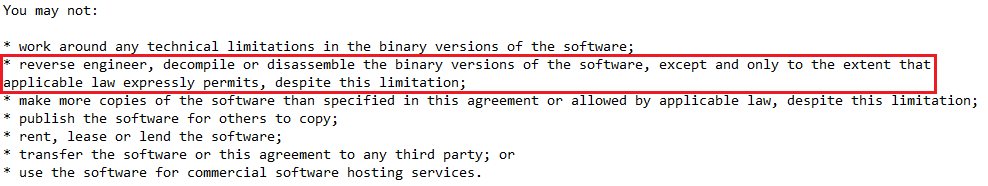
\includegraphics[width=1\textwidth]{reverse_engineering/strings_eula.png}}
	\caption{Part of the EULA bundled with the \textit{strings} application provided by Microsoft.}
	\label{fig:strings_eula}
\end{figure}


